
\begin{center}
      \textbf{CHƯƠNG I: TỔNG QUAN OSA, MỐI LIÊN HỆ VỚI TƯ THẾ NGỦ VÀ
            KĨ THUẬT SÀNG LỌC, PHÂN LOẠI}
\end{center}
Trong chương này, sẽ trình bày tổng quan về hội chứng ngưng thở khi ngủ do tắc
nghẽn, phân tích mối quan hệ của tư thế ngủ đối với mức độ nghiêm trọng của OSA
và dạng OSA ngủ phụ thuộc tư thế. Tiếp đó, chương tập trung làm rõ cơ sở khoa
học cho việc phát triển các thiết bị theo dõi giấc ngủ, phân loại tư thế ngủ
tại nhà. Cuối cùng, đưa ra xu hướng ứng dụng trí tuệ nhân tạo và điện toán biên
trong thu thập, phân tích dữ liệu cảm biến để phân loại tư thế ngủ, qua đó đặt
nền tảng cho các hướng nghiên cứu và triển khai kỹ thuật được trình bày trong
những chương tiếp theo.
\section{Hội chứng ngưng thở khi ngủ}

\subsection{Khái niệm}

Trong số các rối loạn hô hấp liên quan đến giấc ngủ đã đề cập, OSA là dạng phổ
biến nhất và có tác động sâu rộng đến sức khỏe cộng đồng. Mức độ của OSA được
đánh giá dựa trên chỉ số ngưng thở giảm thở (AHI) bằng cách chia tổng số lần
ngưng thở và giảm thở cho tổng số giờ đã ngủ.

\subsection{Nguyên nhân}

Nguyên nhân của OSA đến từ đa dạng các yếu tố bao gồm cả hình thái giải phẫu và
các chức năng sinh lý của đường hô hấp trên. Các nguyên nhân thường không đồng
nhất giữa các người bệnh.

\subsection{Ảnh hưởng của OSA}
Uớc tính có gần một tỷ người trên toàn cầu mắc OSA. Tại Việt Nam, theo
GS.TS.BS. Dương Quý Sỹ \footnote{Giáo sư, Tiến sĩ, Bác sĩ Dương Quý Sỹ là Chủ
      tịch Hội Giấc ngủ Việt Nam, chuyên gia đầu ngành về rối loạn giấc ngủ và hô
      hấp.}, tỷ lệ mắc OSA ở người trưởng thành chiếm khoảng 8,5\%. Hơn nữa, tình
trạng giảm oxy máu liên tục tái diễn trong khi ngủ cùng với sự gián đoạn chu kỳ
giấc ngủ được chứng minh có liên quan mật thiết đến nhiều bệnh lý mãn tính như
suy tim, bệnh động mạch vành, rối loạn nhịp tim, gan nhiễm mỡ do rối loạn
chuyển hóa và đột quỵ.

\subsection{Tư thế ngủ và mối liên hệ với OSA}
Tư thế ngủ giữ vai trò thiết yếu trong việc duy trì sức khỏe tổng thể và chất
lượng giấc ngủ, bên cạnh các yếu tố khác như thời lượng, môi trường và thói
quen ngủ. Nhiều nghiên cứu đã chỉ ra rằng tư thế ngủ có thể ảnh hưởng trực tiếp
đến hoạt động của hệ hô hấp, tim mạch và hệ cơ - xương, đặc biệt là cột sống.

\begin{figure}[H]
      \centering
      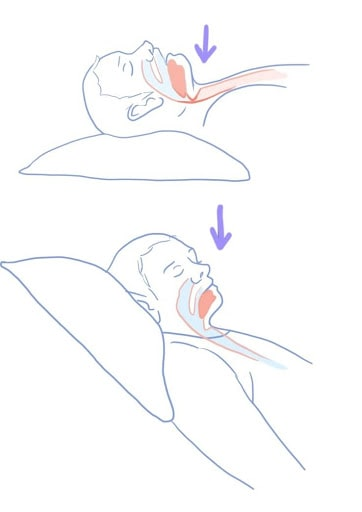
\includegraphics[width=0.3\textwidth]{images/tuthe_osa.png} % giảm xuống 70% chiều rộng trang
      \vspace*{-5mm}
      \caption{Xẹp đường thở ở tư thế ngửa}
      \label{fig:tuthe_osa}
\end{figure}

Trong phạm vi hội chứng ngưng thở tắc nghẽn khi ngủ, tư thế ngủ được xem là một
yếu tố quan trọng quyết định mức độ nghiêm trọng của bệnh. Các nghiên cứu cho
thấy, nhiều bệnh nhân OSA có tần suất ngưng thở và giảm thở cao hơn rõ rệt khi
nằm ngửa so với các tư thế khác. tượng này được gọi là OSA phụ thuộc tư thế.
Định nghĩa sớm nhất là do Cartwright (1984) đưa ra cho rằng bệnh nhân được xem
là mắc pOSA khi chỉ số AHI ở tư thế nằm ngửa cao hơn ít nhất hai lần so với AHI
ở tư thế không nằm ngửa.

\section{Công nghệ trong chẩn đoán OSA và phân loại tư thế ngủ}

\subsection{Đa ký giấc ngủ}
Phương pháp đa ký giấc ngủ (PSG) được xem là tiêu chuẩn vàng trong chẩn đoán
hội chứng ngưng thở khi ngủ. Phương pháp này sẽ ghi lại đa kênh dữ liệu trong
lúc ngủ liên tục suốt một đêm. Tuy nhiên, phương pháp PSG vẫn còn một số hạn
chế về mặt chi phí và sự thuận tiện.

\subsection{Thiết bị theo dõi OSA tại nhà}
Các thiết bị theo dõi tại nhà (HST) được thiết kế với mục tiêu giảm kích thước, chi
phí phù hợp, thuận tiện sử dụng tại nhà. Để làm được điều đó thì các thiết bị
HST cần phải giảm thiểu số lượng cảm biến nhưng vẫn đảm bảo độ chính xác. Điều
này có thể đạt được thông qua việc tích hợp các thuật toán xử lý tín hiệu và mô
hình học máy có thể được thực thi trực tiếp trên phần cứng nhúng hoặc thông qua
ứng dụng hỗ trợ trên điện thoại di động.

\subsection{Kĩ thuật phân loại tư thế ngủ}

Hiện nay, có nhiều nghiên cứu tập trung phát triển các hệ thống theo dõi tư thế
ngủ. Các nghiên cứu này sử dụng: thảm cảm biến áp lực, camera RGB hoặc camera
hồng ngoại, cảm biến gia tốc ở ngay trên chính chiếc điện thoại và cuối cùng
tập trung vào việc tối giản phần cứng, đặc biệt là sử dụng duy nhất một cảm
biến gia tốc để nhận dạng tư thế ngủ. Kết hợp bộ dữ liệu này với các mô hình
học máy cho độ chính xác cao. Hơn nữa, đã có nghiên cứu triển khai trên được
nền tảng nhúng. Tuy nhiên, tại Việt Nam chưa có công bố thực hiện triển khai
bài toán phân loại tư thế ngủ trên biên và có phân tích rõ ràng về hệ thống thu
thập và ý nghĩa của đặc trưng lên mô hình.

\subsection{Cảm biến gia tốc trong đánh giá tư thế ngủ}

Ưu điểm nổi bật của cảm biến gia tốc nằm ở khả năng vận hành độc lập với mức
tiêu thụ năng lượng thấp, đồng thời có thể tích hợp dễ dàng vào các hệ thống
bảng mạch.
Ngoài ra, cảm
biến gia tốc ít phụ thuộc vào các điều kiện môi trường như ánh sáng, nhiệt độ,
sử dụng chăn. Và quan trọng hơn, phương pháp này không xâm phạm quyền riêng tư
của người dùng như các hệ thống giám sát bằng hình ảnh.

\subsection*{Nguyên lý hoạt động cảm biến gia tốc}

Hiện nay, các loại cảm biến gia tốc phổ biến được chế tạo bằng công nghệ vi cơ
điện tử (Micro-Electro-Mechanical Systems - MEMS) với ba kiểu chính là: kiểu áp
điện trở, kiểu điện dung và kiểu áp điện.

\begin{figure}[H]
      \centering
      \[
            \text{Tác động đầu vào}
            \;\xrightarrow[\text{Gây ra dịch chuyển }x]{}
            \;
            \text{Thay đổi điện dung }(\Delta C)
            \;\xrightarrow[\text{Mạch xử lý tín hiệu}]{}
            \;
            \text{Điện áp ra}
      \]
      \caption{Quá trình biến đổi tín hiệu trong cảm biến điện dung.}
      \label{fig:signal_flow}
\end{figure}

\subsection{Học máy trong phân loại OSA và tư thế ngủ}

Cùng với lượng dữ liệu phong phú và liên tục được thu thập từ các cảm biến, các
thuật toán học máy trở thành công cụ để phân tích và khai thác hiệu quả các
dòng dữ liệu này, giúp đưa ra quyết định nhanh chóng và chính xác. Đặc biệt,
trong bối cảnh các thiết bị theo dõi sức khỏe tại nhà yêu cầu kích thước nhỏ
gọn, có khả năng đeo được, không phụ thuộc vào kết nối Internet, thì học máy
tại biên trở thành như một giải pháp tối ưu vừa mang lại khả năng tính toán
mạnh mẽ, vừa dễ dàng triển khai trên các phần cứng có tài nguyên hạn chế.
